\documentclass{standalone}
\usepackage{pgfplots, amssymb}
\pgfplotsset{
  compat=1.18, 
  trig format=rad, 
  ticklabel style = {font=\footnotesize},
  axis equal image,
}

\begin{document}
  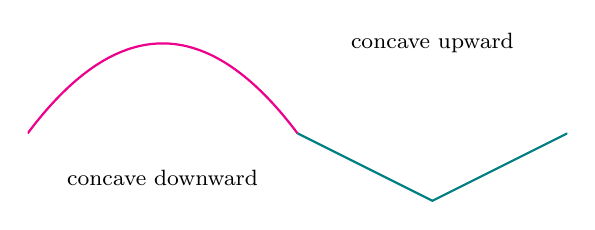
\begin{tikzpicture}
    \begin{axis}[
      axis lines=none,
      samples=500,
      smooth,
      no markers,
      xmin=0, xmax=4,
      % ymin=-1, ymax=5,
      thick,
      ]
      % sage: f(x) = ((x+1)*(x-2)).integrate(x).integrate(x)
      \addplot[magenta, domain=0:2] {(-(2*(x-1))^2/3)/2};
      \node at (1,-1) {\footnotesize concave downward};
      \addplot[teal, domain=2:4] {(abs(x - 3) - (2*(2-1))^2/3 - 1)/2};
      \node at (3,0) {\footnotesize concave upward};
    \end{axis}
  \end{tikzpicture}
\end{document}
